\section{Tatree$<$ Sets\-Type $>$ Class Template Reference}
\label{class_tatree}\index{Tatree@{Tatree}}
Template class representing a trie data structure (this is an \char`\"{}interface\char`\"{} of the Tatre\_\-base class).  


{\tt \#include $<$Tatree.hxx$>$}

Inheritance diagram for Tatree$<$ Sets\-Type $>$::\begin{figure}[H]
\begin{center}
\leavevmode
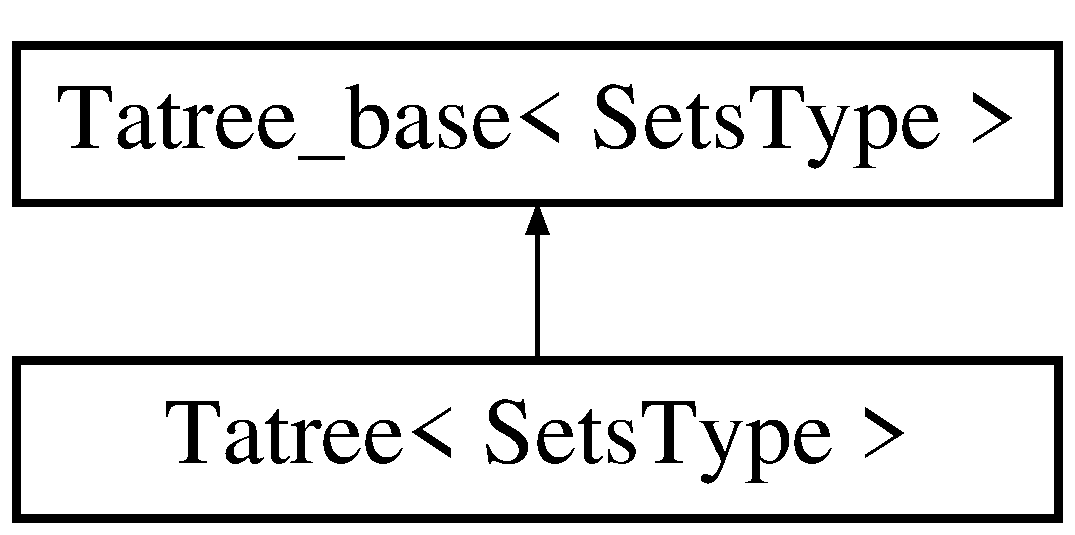
\includegraphics[height=2cm]{class_tatree}
\end{center}
\end{figure}
\subsection*{Public Types}
\begin{CompactItemize}
\item 
typedef {\bf It\-Tatree}$<$ Sets\-Type $>$ {\bf iterator}\label{class_tatree_06094a289a982269a29926e3f22b8356}

\begin{CompactList}\small\item\em Used to have the same syntax tha the STL. \item\end{CompactList}\end{CompactItemize}
\subsection*{Public Member Functions}
\begin{CompactItemize}
\item 
{\bf Tatree} ()\label{class_tatree_7ba7fda13c2987a2840c07164c2d17e6}

\begin{CompactList}\small\item\em Constructor. \item\end{CompactList}\item 
{\bf $\sim$Tatree} ()\label{class_tatree_d54e3fb0fc9525949c010f9290fb97f7}

\begin{CompactList}\small\item\em Destructor. \item\end{CompactList}\item 
{\bf It\-Tatree}$<$ Sets\-Type $>$ {\bf begin} ()\label{class_tatree_383cce0f85279182e9eb5e19015cae0f}

\begin{CompactList}\small\item\em Return an iterator on the first element stored. \item\end{CompactList}\item 
{\bf It\-Tatree}$<$ Sets\-Type $>$ {\bf begin\-Root} ()\label{class_tatree_14ef8d3302fb0d1f520a39b09ba71b65}

\begin{CompactList}\small\item\em Return an iterator on the root node. \item\end{CompactList}\item 
{\bf It\-Tatree}$<$ Sets\-Type $>$ {\bf end} ()\label{class_tatree_7dea4be6a2c8914398d8073189c7e845}

\begin{CompactList}\small\item\em Return an iterator on the element after the last element stored. \item\end{CompactList}\item 
void {\bf print} ()\label{class_tatree_2690856037aef1ae34a711b5f4136069}

\begin{CompactList}\small\item\em Function that print to screen the sets stored in the trie. \item\end{CompactList}\item 
{\bf Tatree\-Node}$<$ Sets\-Type $>$ $\ast$ {\bf get\-Root} ()\label{class_tatree_940b8597e71da99ff8bc673aaad7a53b}

\begin{CompactList}\small\item\em Return the root node. \item\end{CompactList}\item 
void {\bf set\-Recode} ({\bf Recode\-To\-Int}$<$ Sets\-Type $>$ $\ast$inrec)\label{class_tatree_69650ee7743c216a5e4080e2ebaa68a0}

\begin{CompactList}\small\item\em Set the recode functor to the functor passed in parameter. \item\end{CompactList}\item 
{\bf Recode\-To\-Int}$<$ Sets\-Type $>$ $\ast$ {\bf get\-Recode} ()\label{class_tatree_cca02ceb8838b29546f807316b187182}

\begin{CompactList}\small\item\em Get the recode functor. \item\end{CompactList}\end{CompactItemize}
\subsection*{Friends}
\begin{CompactItemize}
\item 
class {\bf It\-Tatree$<$ Sets\-Type $>$}\label{class_tatree_e63ac7816d95fec5ec77b16c2597e4b7}

\end{CompactItemize}


\subsection{Detailed Description}
\subsubsection*{template$<$class Sets\-Type$>$ class Tatree$<$ Sets\-Type $>$}

Template class representing a trie data structure (this is an \char`\"{}interface\char`\"{} of the Tatre\_\-base class). 

This class differs from the mother class {\bf Tatree\_\-base}{\rm (p.\,\pageref{class_tatree__base})} by providing additional methods and the access to a more complete iterator. Using this class, it is possible to explore all the sets stored in trie using the iterators ++. The template parameter is the type of the element stored in the trie. 



The documentation for this class was generated from the following file:\begin{CompactItemize}
\item 
F:/i\-Zi/data\-Structures/trie/Tatree.hxx\end{CompactItemize}
